\section{Parser}
\label{sec:parser}
The scanner \ref{sec:scannertheory} has the purpose to recognize tokens, and that leads to recognizing the input string and determining the phrase structure, which is the purpose of the parser \cite{misc:spo}. We strive to make the language unambiguous\footnote{This means that every sentence has exactly one abstract syntax tree (AST). See section \ref{asttheory} for more about the abstract syntax tree.} to avoid the complication an ambiguous sentence would bring.\\
\\
There are two basic parsing strategies, \textit{bottom-up} and \textit{top-down}. We will here expand on the \textit{top-down} strategy, because that is what we have implemented.\\ \indent
The \textit{top-down} parsing algorithm is characterized by the way it builds the AST. The parser does not \textit{need} to make an AST, but it is convenient to describe the parsing strategy by making the AST. The \textit{top-down} approach consider the terminal symbols of a string, from left to right, and constructs its AST from top to bottom (from root node to terminal node).\\ \indent
Here is an example of how the parser would make an AST:

\begin{figure}[H]
\begin{center}
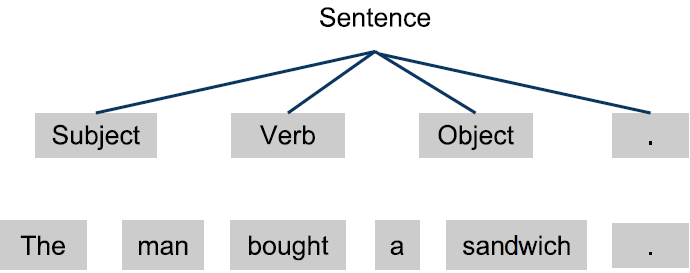
\includegraphics[scale=0.5]{Images/parsingexample/AST1.png}
\end{center}
\caption{The first step for the parser is to decide what to apply ind the root node. Here it has only one option: "Sentence ::= Subject Verb Object."}
\end{figure}

The words that are not shaded are final elements in the AST. The words that are shaded and has a line to the previous node, is called stubs, and are not final elements, because they depend on the terminal nodes. The shaded nodes with no connection lines are the terminal symbols that are not yet examined.

\begin{figure}[H]
\begin{center}
\includegraphics[scale=0.5{Images/parsingexample/AST2.png}
\end{center}
\caption{In the second step the parser looks at the stub to the left. Here the correct production rule is: "Subject ::= \textbf{The} noun".}
\label{fig:ast2}
\end{figure}

The parser chooses the production rules by examining the next input terminal symbol. If the terminal symbol in figure \ref{fig:ast2} had been "A" then it would have chosen the production rule: "Subject ::= \textbf{A} noun".

\begin{figure}[H]
\begin{center}
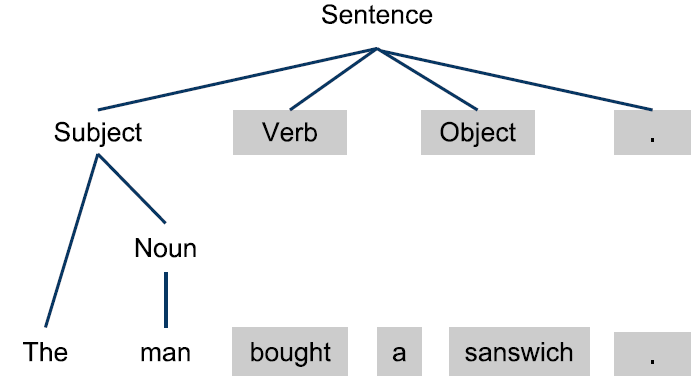
\includegraphics[scale=0.5]{Images/parsingexample/AST3.png}
\end{center}
\caption{In third step the noun-stub is concidered, and the production rule becomes: "Noun ::= man".}
\end{figure}

\begin{figure}[H]
\begin{center}
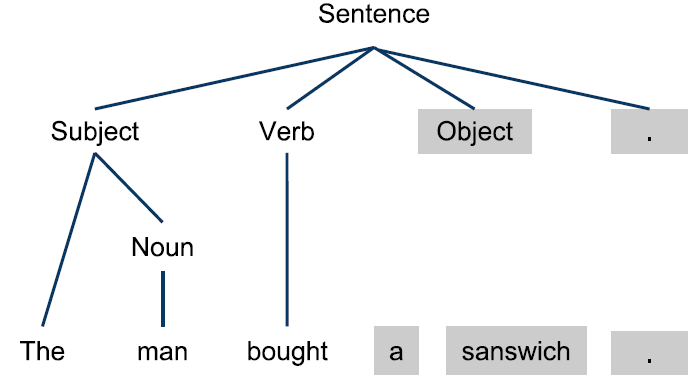
\includegraphics[scale=0.5]{Images/parsingexample/AST4.png}
\end{center}
\caption{In fourth step the verb-stub is concidered, and the production rule becomes: "Verb ::= bought".}
\end{figure}

\begin{figure}[H]
\begin{center}
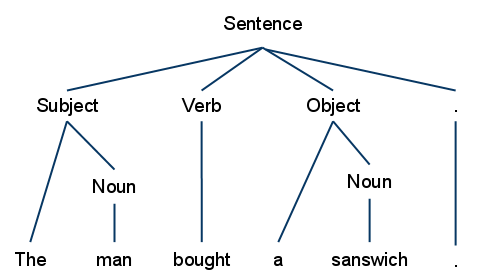
\includegraphics[scale=0.5]{Images/parsingexample/AST5.png}
\end{center}
\caption{Here is the final syntax tree when the parser is done.}
\end{figure}

This method is continued until the whole sentence has been parsed. Here the final syntax tree is quite simpel, but one can imagine how the tree will grow when the input is a larger program text. See section \ref{AST} on how we have implemented the AST.
